\let\negmedspace\undefined
\let\negthickspace\undefined
\documentclass[journal,12pt,twocolumn]{IEEEtran}
\usepackage{cite}
\usepackage{amsmath,amssymb,amsfonts,amsthm}
\usepackage{algorithmic}
\usepackage{graphicx}
\usepackage{textcomp}
\usepackage{xcolor}
\usepackage{txfonts}
\usepackage{listings}
\usepackage{enumitem}
\usepackage{mathtools}
\usepackage{gensymb}
\usepackage{comment}
\usepackage[breaklinks=true]{hyperref}
\usepackage{tkz-euclide} 
\usepackage{listings}
\usepackage{gvv}                                        
\def\inputGnumericTable{}                                 
\usepackage[latin1]{inputenc}                                
\usepackage{color}                                            
\usepackage{array}                                            
\usepackage{longtable}                                       
\usepackage{calc}                                             
\usepackage{multirow}                                         
\usepackage{hhline}                                           
\usepackage{ifthen}                                           
\usepackage{lscape}
\newtheorem{theorem}{Theorem}[section]
\newtheorem{problem}{Problem}
\newtheorem{proposition}{Proposition}[section]
\newtheorem{lemma}{Lemma}[section]
\newtheorem{corollary}[theorem]{Corollary}
\newtheorem{example}{Example}[section]
\newtheorem{definition}[problem]{Definition}
\newcommand{\BEQA}{\begin{eqnarray}}
\newcommand{\EEQA}{\end{eqnarray}}
\newcommand{\define}{\stackrel{\triangle}{=}}
\theoremstyle{remark}
\newtheorem{rem}{Remark}
\begin{document}
\bibliographystyle{IEEEtran}
\vspace{3cm}
\title{\textbf{11.9.3.2}}
\author{EE23BTECH11040-MANOJ KUMAR AMBATIPUDI$^{*}$% <-this % stops a space
}
\maketitle
\newpage
\bigskip
\renewcommand{\thefigure}{\theenumi}
\renewcommand{\thetable}{\theenumi}
\textbf{QUESTION:}\\\\
Find the $12^{th}$ term of a G.P. whose $8^{th}$ term is 192 and common ratio is 2.\\\\
\textbf{SOLUTION:}\\
The general term of a G.P. is $a_0r^{n}$ where $a_0$ is the first term, r is the common difference and n is the number indicating $\brak{n+1}^{th}$ term of the sequence.
\begin{align}
    \implies a_n=a_0r^{n}
\end{align}
Given, $a_7=192$, $r=2$. On substituting, we get
\begin{align}
\implies a_02^{7}&=192\\
\implies 128a_0&=192\\
\implies\boxed{a_0=\dfrac{3}{2}=1.5}
\end{align}
Therefore, on substituting back, we get
\begin{align}
    a_n=1.5\times2^{n}
\end{align}
\begin{align}
\therefore a_{11} = 1.5\times2^{11} = 3072
\end{align}
\begin{figure}[h]
\renewcommand\thefigure{1} 
    \centering
    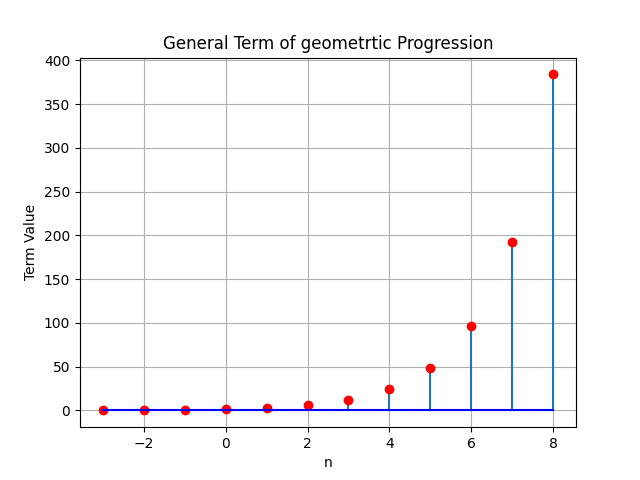
\includegraphics[width=1.0\linewidth]{Figure_3.png}
    \caption{Plot of the general term taken from Python}
    \label{fig:1}
\end{figure}\\
General term can also be written as\
\begin{align}
\boxed{x\brak{n} = 1.5\times2^{n}u\brak{n}}
\end{align}\
Now on Z-Transforming, the expression which we get is\\
\begin{align}
X\brak{z} &= \sum_{-\infty}^{\infty}1.5\times2^{n}z^{-n}u(n)   \\
\implies X\brak{z} &= \sum_{-\infty}^{\infty}1.5\times\brak{\dfrac{2}{z}}^{n}u(n)
\end{align}
For the above series to converge, modulus of common ratio should be less than 1.
\begin{align}
\implies r &= \bigg|\dfrac{2}{z}\bigg|<1\\
 \implies       |z|&> 2
\end{align}
Therefore for all values given above, the above sequence shall converge.\\
The expression of $x\brak{n}$ is 
\[
u\brak{n}=
\begin{cases}
    1,&\,\,\,\forall\,\,\,n>0\\
    0,&\,\,\,\forall\,\,\,n<0
\end{cases}
\]
On simplifying $X\brak{z}$, we get
\begin{align}
\boxed{X\brak{z}=\dfrac{3}{z-2}u(z)}\,\,\,  \forall \,\,\, |z|>2 
\end{align}
The expression of u\brak{z} is 
\[
u\brak{z}=
\begin{cases}
    0,&\,\,\,\forall\,\,\,z<0,z \in Z\\
    1,&\,\,\,\forall\,\,\,z>0,z \in Z
\end{cases}
\]
Now the expression simplifies to
\begin{align}
   \boxed{X\brak{z}=\dfrac{3}{z-2}}\,\,\, \forall \,\,\, z>2
\end{align}
\begin{table}[ht]
\renewcommand\thetable{1} 
    \centering
    \begin{tabular}{|c|c|c|}
    \hline
        Variable&Description&value\\\hline
        $a_0$&First Term in G.P.&1.5\\\hline
        n&Describing the order of term&None\\\hline
        $a_7$&$8^{th}$ term&192\\\hline
        $r$&common ratio&2\\\hline
        $a_{11}$&$12^{th}$ term&3072\\\hline
        x\brak{n}&General term of sequence&None\\\hline
        u\brak{n},u\brak{z}&Unit Step Functions&Given Before\\\hline
        X\brak{z}&Z-Transform Equation&None\\\hline
        z&frequency&None\\\hline
    \end{tabular}
    \vspace{0.3cm}
    \caption{VARIABLES USED}
    \label{tab:my_label}
\end{table}
\end{document}
